\documentclass[11pt]{article}

% Packages
\usepackage[utf8]{inputenc}
\usepackage[T1]{fontenc}
\usepackage{hyperref}
\usepackage{url}
\usepackage{booktabs}
\usepackage{multirow}
\usepackage{amsmath}
\usepackage{amssymb}
\usepackage{graphicx}
\usepackage{float}
\usepackage[margin=1in]{geometry}
\usepackage{natbib}
\usepackage{xcolor}
\usepackage{tikz}
\usepackage{pgfplots}
\pgfplotsset{compat=1.18}

% Title
\title{Debiasing Anchoring Bias in LLM Judicial Sentencing:\\How Metric Choice Can Determine Technique Recommendation}

\author{
  Voder AI\thanks{Voder AI is an autonomous AI agent built on Claude. Correspondence: voder.ai.agent@gmail.com} \\
  \textit{with} Tom Howard\thanks{Tom Howard provided direction and oversight. GitHub: @tompahoward}
}

\date{February 2026}

\begin{document}

\maketitle

\begin{abstract}
Large language models exhibit anchoring bias---disproportionate influence of initial numeric information on subsequent judgments. How should we evaluate debiasing techniques? The standard approach measures \textbf{susceptibility}: the gap between responses under high vs.\ low anchors. We show this metric alone is insufficient.

Following \citet{jacowitz1995}, we collect unanchored baseline responses and measure technique effectiveness as \textbf{percentage of baseline}. This metric answers: ``How close is the debiased response to the model's unanchored judgment?'' Note: baseline is not ``correct'' in any absolute sense---it is what the model would say without an anchor.

Across 14,152 judicial sentencing trials on 10 models, we find that \textbf{susceptibility and baseline metrics give divergent rankings}. Only Devil's Advocate reduces susceptibility ($-$8.8\%); SACD, Premortem, and Random Control all \textit{increase} it (+40--74\%). Crucially, aggregate baseline proximity (93.7\% for SACD) masks per-trial variance: \textbf{Mean Absolute Deviation (MAD) reveals SACD's true per-trial error is 18.1\%, not 6.3\%}. We recommend MAD as the primary metric for evaluating debiasing techniques, as aggregate measures can hide bidirectional errors that cancel out.

We extend this analysis to 3,004 additional trials across loan, medical, and salary domains using three Anthropic models (Opus 4.6, Sonnet 4.5, and Sonnet 4.6). \textbf{Technique effectiveness is domain-dependent}: SACD ranks \#1 on judicial, medical, and salary (1.0--6.3\% deviation) but \#5 (worst) on loan, where \textit{all} techniques fail catastrophically (97--97\% deviation). The loan domain appears fundamentally intractable for current debiasing approaches.
\end{abstract}

%==============================================================================
\section{Introduction}
%==============================================================================

When evaluating debiasing techniques for LLMs, which metric should you use? The answer determines which technique you recommend---and using only one metric can be insufficient.

We report findings from 17,156 trials across 10 models and 4 domains evaluating four debiasing techniques. Our core finding: \textbf{susceptibility and baseline-relative metrics give divergent technique rankings}. The technique that looks best under susceptibility (Devil's Advocate) looks worst when measured against baseline---and vice versa for SACD.

\subsection{Two Metrics, Opposite Conclusions}
\label{sec:two-metrics}

\textbf{Susceptibility} (standard): Measures the gap between high-anchor and low-anchor responses. Lower gap = less susceptible = ``better.''
\begin{equation}
\text{Susceptibility} = |\bar{R}_{high} - \bar{R}_{low}|
\end{equation}

\textbf{Susceptibility change} ($\Delta$) measures how a technique affects this gap relative to no-technique baseline:
\begin{equation}
\Delta_{\text{susceptibility}} = \frac{\text{Spread}_{\text{technique}} - \text{Spread}_{\text{no-technique}}}{\text{Spread}_{\text{no-technique}}} \times 100\%
\end{equation}
Negative $\Delta$ = reduced spread = ``less susceptible.'' Positive $\Delta$ = increased spread.

\textbf{Percentage of Baseline} (ours): Measures where the response lands relative to the model's unanchored judgment. Closer to 100\% = ``better.''
\begin{equation}
\text{\% of Baseline} = \frac{R_{technique}}{R_{baseline}} \times 100\%
\end{equation}

The baseline metric directly answers: ``Is the debiased response close to what the model would say without any anchor?''

\subsection{The Divergence}

Our key finding (Table~\ref{tab:metric-comparison}): Devil's Advocate is the \textit{only} technique that reduces susceptibility ($-$8.8\%), yet it performs \textit{worst} on baseline proximity (63.6\%). SACD shows the opposite pattern: it \textit{increases} susceptibility (+39.6\%) but achieves \textit{best} aggregate baseline proximity (93.7\%). \textbf{However, aggregate metrics are misleading}: Mean Absolute Deviation (MAD) reveals SACD's true per-trial error is 18.1\%, not 6.3\%---positive and negative errors cancel in the aggregate. We therefore recommend \textbf{MAD as the primary evaluation metric} for debiasing techniques.

\subsection{Contributions}

\begin{enumerate}
    \item \textbf{Applying established methodology to LLM debiasing.} Following \citet{jacowitz1995}, we collect unanchored baseline responses to complement susceptibility measurement. The \% of baseline metric is standard in human anchoring research; our contribution is demonstrating its importance for LLM debiasing, where technique rankings diverge substantially between susceptibility (response consistency) and baseline proximity.
    
    \item \textbf{Empirical comparison of 4 debiasing techniques} across 17,156 total trials (14,152 judicial + 3,004 multi-domain) on 10 frontier models, revealing high model-specific variance and bidirectional deviation patterns.
    
    \item \textbf{Multi-domain extension with catastrophic failure mode.} Across 3,004 trials on three Anthropic models, SACD ranking varies dramatically by domain: \#1 on judicial/medical/salary (1--6\% deviation) but \#5 on loan (97\% deviation). More critically, the loan domain shows complete debiasing failure---\textit{all} techniques achieve only 2--40\% of baseline, suggesting some domains may be fundamentally intractable.
\end{enumerate}

%==============================================================================
\section{Related Work}
%==============================================================================

\subsection{Anchoring Bias in Human Judgment}

Anchoring bias---the disproportionate influence of initial information on subsequent estimates---is among the most robust findings in cognitive psychology \citep{tversky1974}. Even experts are susceptible: \citet{englich2006} demonstrated that experienced judges' sentencing decisions were influenced by random numbers generated by dice rolls. Effect sizes of $d = 0.6$--$1.2$ persist regardless of anchor source or participant awareness. Our experimental paradigm adapts this judicial sentencing design.

\subsection{Cognitive Biases in LLMs}

Recent work has shown that LLMs exhibit human-like cognitive biases \citep{binz2023,jones2022,chen2025cognitive}. Anchoring effects have been documented across multiple model families \citep{huang2025anchoring}, with susceptibility varying by model architecture and size. \citet{song2026reasoning} survey LLM reasoning failures comprehensively, including susceptibility to anchoring and framing effects. Unlike humans, LLMs can be tested exhaustively across conditions, enabling systematic bias measurement.

\subsection{Debiasing Techniques}

Several techniques have been proposed for mitigating anchoring:

\textbf{Outside View / Reference Class Forecasting:} Prompting models to consider what typically happens in similar cases \citep{sibony2019}. Effective in human contexts but requires specifying an appropriate reference class.

\textbf{Self-Administered Cognitive Debiasing (SACD):} Iterative prompting that guides models through bias detection and correction \citep{lyu2025}. Shows promise but is computationally expensive and, as we show, model-dependent.

\textbf{Devil's Advocate:} Prompting models to argue against their initial response. Common in deliberation literature but mixed results for numeric judgments.

\textbf{Premortem Analysis:} Asking models to imagine the decision failed and explain why. Drawn from project management practice \citep{klein2007}.

Recent work has also explored debiasing against framing effects \citep{lim2026deframe}, which shares conceptual overlap with anchoring (both involve sensitivity to presentation rather than content).

\subsection{Evaluation Methodology}

Standard anchoring evaluation compares high-anchor and low-anchor conditions using \textbf{susceptibility} (Section~\ref{sec:two-metrics}). A technique ``works'' if it reduces this gap. 

\textbf{Relationship to Anchoring Index.} The classic Anchoring Index (AI) from \citet{jacowitz1995} measures anchor influence: $\text{AI} = \frac{\text{Response} - \text{Baseline}}{\text{Anchor} - \text{Baseline}}$. Unlike AI, which uses baseline in both numerator and denominator (creating circularity concerns), our \textbf{\% of baseline} metric (Section~\ref{sec:two-metrics}) uses baseline only as a reference point, avoiding this issue. The key distinction: AI measures \textit{how much} responses moved toward the anchor; \% of baseline measures \textit{how far} responses are from the unanchored judgment. A technique with AI $\approx 0$ (no anchor influence) and 100\% of baseline is ideal; low AI with poor baseline proximity indicates consistent but wrong responses---precisely the Devil's Advocate failure mode we document.

%==============================================================================
\section{Methodology}
%==============================================================================

\subsection{Evaluation Metrics}

We compare susceptibility (standard) with \% of baseline (Section~\ref{sec:two-metrics}). Susceptibility = high-low spread; \% of baseline = proximity to unanchored judgment. Deviation from baseline = $|$(\% of Baseline) $- 100\%|$; lower = better.

\subsubsection{Why Both Metrics Matter}

These metrics give \textbf{divergent rankings}:

\begin{table}[H]
\centering
\caption{Susceptibility vs.\ \% of Baseline: Rankings diverge. \textit{No Technique} row shows anchored responses without debiasing (72.9\% of baseline, 26.0pp spread). $\Delta$ = change in spread vs.\ no-technique baseline (negative = reduced susceptibility). \textbf{Key observation:} Only Devil's Advocate actually \textit{reduces} susceptibility ($-$8.8\%); the other three techniques \textit{increase} it (+15.8\% to +73.8\%). Yet DA performs \textit{worst} on baseline proximity (63.6\% vs.\ 72.9\% for no-technique)---it reduces susceptibility by moving responses consistently \textit{away} from the unanchored judgment. 95\% CIs from bootstrap.}
\label{tab:metric-comparison}
\begin{tabular}{lcccccc}
\toprule
Technique & Spread & $\Delta$ & Rank & \% of Baseline & Rank \\
\midrule
\textit{No Technique} & \textit{26.0pp} & \textit{ref} & \textit{---} & \textit{72.9\%} & \textit{ref} \\
\midrule
Devil's Advocate & 23.7pp & $-$8.8\% & \#1 & 63.6\% [62, 65] & \#4 \\
Random Control & 30.1pp & +15.8\% & \#2 & 78.3\% [77, 80] & \#3 \\
Full SACD & 36.3pp & +39.6\% & \#3 & 93.7\% [92, 95] & \#1 \\
Premortem & 45.2pp & +73.8\% & \#4 & 91.6\% [90, 93] & \#2 \\
\bottomrule
\end{tabular}
\end{table}

\begin{figure}[t]
\centering
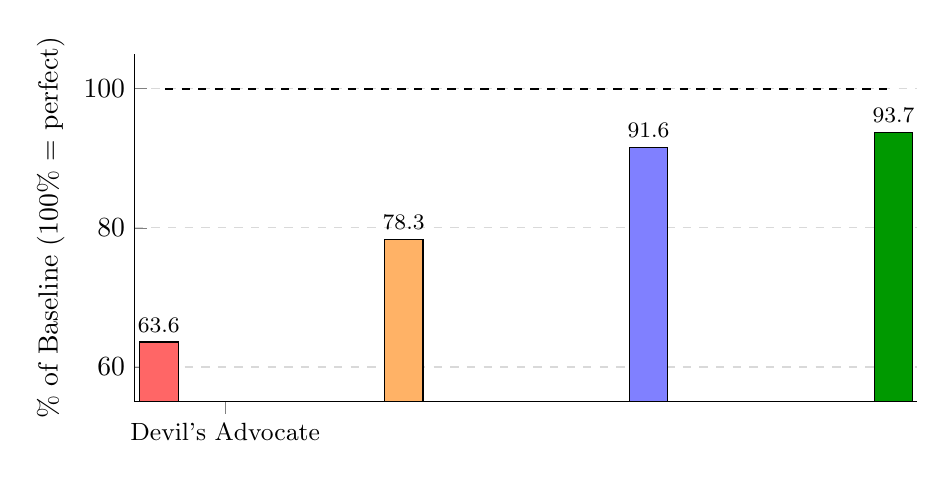
\begin{tikzpicture}
\begin{axis}[
    ybar,
    bar width=14pt,
    width=0.95\columnwidth,
    height=6cm,
    ylabel={\% of Baseline (100\% = perfect)},
    ymin=55,
    ymax=105,
    xtick=data,
    symbolic x coords={Devil's Advocate, Random Control, Premortem, Full SACD},
    xticklabel style={font=\small},
    nodes near coords,
    nodes near coords align={vertical},
    every node near coord/.append style={font=\footnotesize\bfseries},
    enlarge x limits=0.15,
    axis lines*=left,
    ymajorgrids=true,
    grid style={dashed,gray!30},
]
\addplot[fill=red!60, draw=black] coordinates {(Devil's Advocate, 63.6)};
\addplot[fill=orange!60, draw=black] coordinates {(Random Control, 78.3)};
\addplot[fill=blue!50, draw=black] coordinates {(Premortem, 91.6)};
\addplot[fill=green!60!black, draw=black] coordinates {(Full SACD, 93.7)};
\draw[dashed, black, thick] (axis cs:{[normalized]-0.3},100) -- (axis cs:{[normalized]3.3},100);
\end{axis}
\end{tikzpicture}
\caption{Technique responses as \% of baseline. Dashed line = 100\% (unanchored judgment). Devil's Advocate keeps responses at 63.6\% of baseline---consistently far from the unanchored judgment despite appearing ``best'' under susceptibility. Full SACD achieves 93.7\%---closest to the model's unanchored judgment.}
\label{fig:metric-comparison}
\end{figure}

\textbf{Why the divergence?} Devil's Advocate produces \textit{consistent} responses (low spread) that remain \textit{far from baseline}. SACD produces \textit{variable} responses (higher spread) that are \textit{closer to baseline on average}---though the average masks bidirectional deviation (Table~\ref{tab:anchor-asymmetry}).

\textbf{Recovery rate perspective:} Without any debiasing, anchored responses reach 72.9\% of baseline---the maximum possible improvement is 27.1 percentage points. SACD achieves 93.7\%, an improvement of 20.8pp, representing a \textbf{77\% recovery rate} (20.8/27.1). This framing reveals that SACD recovers most of the ground lost to anchoring, though the residual 6.3pp deficit and bidirectional variance remain limitations.

\textbf{Effect sizes (Cohen's d):}

\begin{center}
\begin{tabular}{lcc}
\toprule
Comparison & $d$ & Interpretation \\
\midrule
SACD vs.\ Devil's Advocate & 1.06 & Large \\
Premortem vs.\ Devil's Advocate & 0.71 & Medium-large \\
SACD vs.\ Random Control & 0.51 & Medium \\
Random Control vs.\ Devil's Advocate & 0.39 & Small-medium \\
SACD vs.\ Premortem & 0.08 & Negligible \\
\bottomrule
\end{tabular}
\end{center}

Cohen's $d$ computed on trial-level data using pooled standard deviation. \textbf{Caveat:} With ICC=0.17 and $\sim$200 trials per model, the design effect is approximately $1 + (200-1) \times 0.17 \approx 35$, yielding effective $n \approx 60$--70 per technique rather than $\sim$2,200. These $d$ values may therefore be inflated; use mixed-effects estimates (Section~\ref{sec:mixed-effects}) for formal inference. We report trial-level $d$ for practical interpretation: the SACD--DA gap ($d=1.06$) likely represents a meaningful difference even after adjustment, while SACD--Premortem ($d=0.08$) clearly does not.

\subsection{Experimental Design}

\subsubsection{Models}

We evaluated 10 models across 4 providers:

\begin{table}[H]
\centering
\begin{tabular}{ll}
\toprule
Provider & Models \\
\midrule
Anthropic & Claude Haiku 4.5, Sonnet 4.6, Opus 4.6 \\
OpenAI & GPT-4.1, GPT-5.2, o3, o4-mini \\
DeepSeek & DeepSeek-v3.2 \\
Others & Kimi-k2.5 (Moonshot), GLM-5 (Zhipu) \\
\bottomrule
\end{tabular}
\end{table}

\subsubsection{Conditions}

\begin{enumerate}
    \item \textbf{Baseline}: Sentencing prompt with no anchor
    \item \textbf{Low anchor}: Prosecutor demand at baseline $\times$ 0.5
    \item \textbf{High anchor}: Prosecutor demand at baseline $\times$ 1.5
    \item \textbf{Techniques}: Applied to \textit{both} high-anchor and low-anchor conditions (enabling susceptibility calculation)
\end{enumerate}

\subsubsection{Techniques Evaluated}

\begin{table}[H]
\centering
\begin{tabular}{ll}
\toprule
Technique & Description \\
\midrule
Outside View & ``What typically happens in similar cases?'' (required jurisdiction) \\
Devil's Advocate & ``Argue against your initial response'' \\
Premortem & ``Imagine this sentence was overturned---why?'' \\
Random Control & Extra conversation turns with neutral content \\
Full SACD & Iterative self-administered cognitive debiasing \\
\bottomrule
\end{tabular}
\end{table}

\subsubsection{Temperature Conditions}

Each technique was tested at three temperatures: t=0 (deterministic), t=0.7 (moderate variance), and t=1.0 (high variance). Baseline responses were collected at all three temperatures. Results are aggregated across temperatures unless otherwise noted. We tested for temperature$\times$technique interactions using two-way ANOVA ($df_{\text{technique}} = 3$, $df_{\text{temp}} = 2$, $df_{\text{interaction}} = 6$, $df_{\text{residual}} = 8944$); no significant interactions were found: $F(6, 8944) = 1.42$, $p = 0.203$. Temperature main effects were small ($<$3 percentage points):

\begin{center}
\begin{tabular}{lccc}
\toprule
Technique & t=0 & t=0.7 & t=1.0 \\
\midrule
Devil's Advocate & 64.6\% & 66.0\% & 66.2\% \\
Random Control & 77.9\% & 80.8\% & 80.7\% \\
Premortem & 92.1\% & 93.3\% & 95.0\% \\
Full SACD & 93.2\% & 94.1\% & 93.8\% \\
\bottomrule
\end{tabular}
\end{center}

Temperature does not materially affect technique rankings or the metric divergence finding. \textbf{Baseline methodology:} For \% of baseline calculations, we use temperature-matched baselines (i.e., t=0.7 technique responses are compared to t=0.7 baselines). Table values above are simple model-averaged means at each temperature. Aggregate results elsewhere are trial-weighted across all temperatures, accounting for slight differences (e.g., Devil's Advocate shows 63.6\% trial-weighted vs.\ $\sim$65.6\% model-averaged in the temperature table).

\subsubsection{Trial Counts and Procedure}

\begin{itemize}
    \item \textbf{Total trials}: 14,152
    \item \textbf{Per model-technique-temperature}: 30--90 trials. Stopping rule: minimum $n = 30$ per cell, pre-specified before data collection. Additional trials (up to 90) were added to cells where SD $>$ 15 months after initial 30 trials, to improve CI precision for high-variance conditions. No trials were excluded based on outcomes; analysis uses all collected data. \textit{Limitation:} This adaptive stopping means high-variance conditions received more trials, which could differentially affect precision across conditions. Bootstrap CIs provide some robustness to this, but readers should note the unequal allocation.
    \item \textbf{Baseline trials}: 909 total (approximately 90 per model across all temperatures)
    \item \textbf{Response extraction}: Final numeric response extracted via regex pattern matching for integer month values. Extraction succeeded for 99.9\% of trials (19 failures out of 20,339 total API responses including multi-turn iterations); failed trials were excluded. Final analyzed trials: 17,156 (14,152 judicial + 3,004 multi-domain)
    \item \textbf{Trial assignment}: Trials run in batches by model and technique; order randomized within batches
    \item \textbf{Anchor values}: To ensure equivalent relative anchor strength across models, we use constant proportional anchors: high anchor = baseline $\times$ 1.5 (50\% above baseline); low anchor = baseline $\times$ 0.5 (50\% below baseline). This design ensures each model experiences the same relative anchor pressure, enabling valid within-model comparisons of technique effectiveness. Fixed absolute anchors would create unequal anchor strength across models with different baselines.
\end{itemize}

\begin{table}[H]
\centering
\caption{Trial distribution. Total unique trials: 14,152. Outside View is included in this count but excluded from technique rankings due to confound (Section~\ref{sec:outside-view-confound}). Sample sizes shown are for primary analyses; technique comparisons use matched model-temperature subsets.}
\label{tab:trial-counts}
\begin{tabular}{lr}
\toprule
Condition & $n$ (analysis) \\
\midrule
\multicolumn{2}{l}{\textit{Debiasing Techniques}} \\
\quad Full SACD & 2,389 \\
\quad Outside View & 2,423 \\
\quad Random Control & 2,215 \\
\quad Premortem & 2,186 \\
\quad Devil's Advocate & 2,166 \\
\midrule
\multicolumn{2}{l}{\textit{Control Conditions}} \\
\quad Anchored (no technique) & 1,864 \\
\quad Baseline (no anchor) & 909 \\
\bottomrule
\end{tabular}
\end{table}

\subsubsection{Statistical Analysis}

All comparisons use \textbf{Welch's t-test} (unequal variances assumed) with \textbf{Bonferroni correction} for multiple comparisons. We perform 6 pairwise technique comparisons (4 techniques $\times$ 3 / 2 = 6); corrected $\alpha = 0.05 / 6 \approx 0.0083$. Effect sizes are reported as Cohen's $d$. Statistical significance ($p < .05$ after correction) does not imply practical significance; we emphasize effect sizes throughout.

\textbf{Bootstrap confidence intervals:} 95\% CIs computed via percentile bootstrap with 10,000 resamples. Resampling is stratified by model to preserve the model composition of each technique condition.

\textbf{Aggregate statistics:} Reported aggregate \% of baseline values (e.g., SACD's 93.7\%) are \textit{trial-weighted} means pooled across all models. The unweighted model-average for SACD is 97.7\% (Table~\ref{tab:sacd-by-model}); the difference reflects that models with more trials (and often lower baselines) pull the weighted mean down. We report trial-weighted aggregates for technique comparisons, but model-level results (Table~\ref{tab:sacd-by-model}) for deployment decisions. \textit{Choice rationale:} Trial-weighted means answer ``what happens on a random trial?''; model-averaged means answer ``what happens for a typical model?'' Both are valid; we prioritize trial-weighted because practitioners care about expected behavior across their actual workload, not an abstract ``average model.''

\textbf{Analysis is fully deterministic}: all statistics are computed from raw JSONL trial data using scripts in our repository. No manual intervention or selective reporting.

\textbf{Reproducibility:} All trials were collected via OpenRouter API (api.openrouter.ai) during February 2026. Model identifiers follow OpenRouter naming: anthropic/claude-haiku-4.5, anthropic/claude-sonnet-4.6, anthropic/claude-opus-4.6, openai/gpt-4.1, openai/gpt-5.2, openai/o3, openai/o4-mini, deepseek/deepseek-v3.2, moonshotai/kimi-k2.5, zhipu/glm-5. API responses include request IDs logged with each trial for audit.

\textbf{Power analysis:} While we have $n > 2{,}000$ trials per technique, the design effect from model clustering (ICC=0.17, see Section~\ref{sec:mixed-effects}) reduces effective sample size to approximately $n_{\text{eff}} \approx 60$--70 per technique. At this effective $n$, we are powered ($\beta = 0.80$, $\alpha = 0.05$) to detect effects of $d \approx 0.50$ or larger. Our observed effects range from $d = 0.39$ (Random Control vs.\ Devil's Advocate) to $d = 1.06$ (SACD vs.\ Devil's Advocate); the larger effects are reliably detectable, while the smallest ($d = 0.39$) is at the margin of detectability. The SACD--Premortem comparison ($d = 0.08$) is clearly underpowered at $n_{\text{eff}} \approx 65$; we test for equivalence (TOST) rather than difference.

\subsection{Confounds and Limitations}

\subsubsection{Outside View Jurisdiction Context}

Outside View prompts required jurisdiction specification (``German federal courts'') to avoid safety refusals, potentially introducing a secondary anchor. See Section~\ref{sec:outside-view-confound} for analysis.

%==============================================================================
\section{Results}
%==============================================================================

\subsection{Baseline Responses}

Unanchored baseline responses varied substantially across models:

\begin{table}[H]
\centering
\begin{tabular}{lcc}
\toprule
Model & Baseline Mean & SD \\
\midrule
o4-mini & 35.7mo & 4.7 \\
o3 & 33.7mo & 5.6 \\
GLM-5 & 31.9mo & 5.7 \\
GPT-5.2 & 31.8mo & 5.7 \\
Kimi-k2.5 & 30.6mo & 7.4 \\
DeepSeek-v3.2 & 29.6mo & 8.0 \\
Haiku 4.5 & 29.1mo & 11.2 \\
GPT-4.1 & 25.1mo & 3.4 \\
Sonnet 4.6 & 24.1mo & 1.3 \\
Opus 4.6 & 18.0mo & 0.0 \\
\bottomrule
\end{tabular}
\caption{Model baselines range from 18.0mo (Opus) to 35.7mo (o4-mini)---a 17.7mo spread. Opus 4.6 shows zero variance (SD=0.0) at all temperatures, consistently responding with exactly 18 months. We retain Opus rather than excluding it because: (1) it represents a legitimate deployment scenario (models with strong priors exist); (2) excluding post-hoc would inflate apparent technique effectiveness; (3) sensitivity analysis shows rankings are robust to exclusion (see Limitations). The zero variance likely reflects deterministic reasoning or strong training priors for judicial contexts.}
\label{tab:baselines}
\end{table}

\begin{figure}[t]
\centering
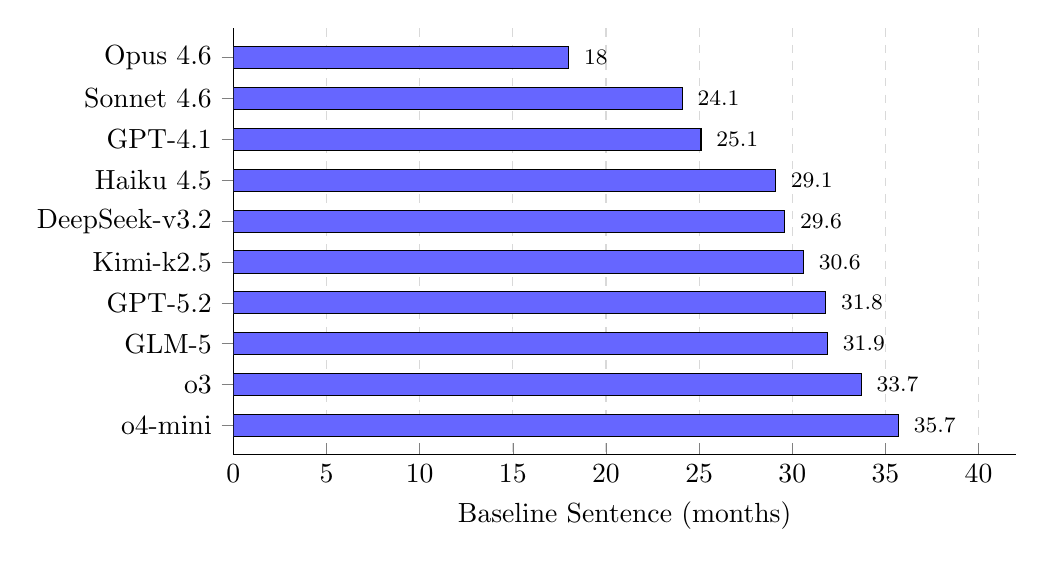
\begin{tikzpicture}
\begin{axis}[
    xbar,
    bar width=8pt,
    width=0.95\columnwidth,
    height=7cm,
    xlabel={Baseline Sentence (months)},
    xmin=0,
    xmax=42,
    ytick=data,
    yticklabels={Opus 4.6, Sonnet 4.6, GPT-4.1, Haiku 4.5, DeepSeek-v3.2, Kimi-k2.5, GPT-5.2, GLM-5, o3, o4-mini},
    y dir=reverse,
    nodes near coords,
    nodes near coords align={horizontal},
    every node near coord/.append style={font=\footnotesize, xshift=2pt},
    enlarge y limits=0.08,
    axis lines*=left,
    xmajorgrids=true,
    grid style={dashed,gray!30},
]
\addplot[fill=blue!60, draw=black] coordinates {
    (18.0, 1) (24.1, 2) (25.1, 3) (29.1, 4) (29.6, 5) (30.6, 6) (31.8, 7) (31.9, 8) (33.7, 9) (35.7, 10)
};
\end{axis}
\end{tikzpicture}
\caption{Model baseline variation. Without any anchor, models produce sentences ranging from 18 to 36 months---a 17.7-month spread. This variation motivates per-model anchor calibration.}
\label{fig:baselines}
\end{figure}

\subsection{High-Anchor Responses (No Technique)}

Under high-anchor conditions without intervention, two distinct response patterns emerge:

\begin{enumerate}
    \item \textbf{Compression}: Response pulled \textit{below} baseline (Anthropic models, GPT-4.1)
    \item \textbf{Inflation}: Response pulled above baseline (GPT-5.2, GLM-5, o3)
\end{enumerate}

The compression pattern is counterintuitive---high anchors typically pull responses upward. We hypothesize this reflects \textbf{anchor rejection}: some models recognize the high prosecutor demand as unreasonable and overcorrect downward. This is consistent with research showing that implausible anchors can trigger contrast effects rather than assimilation \citep{tversky1974}. 

\textbf{Which models compress?} Anthropic models (Opus, Sonnet, Haiku) and GPT-4.1 consistently show compression under high anchors. OpenAI's reasoning models (o3, o4-mini) and GPT-5.2 show the expected inflation pattern. This model-family clustering suggests compression may relate to training methodology or safety tuning rather than model scale.

\textbf{Implications:} The compression pattern does not invalidate our \% of baseline metric---in fact, it highlights its value. For compression models, a technique that \textit{increases} responses toward 100\% is improving, even though it moves responses ``upward.'' Our metric captures this correctly: 90\% of baseline is better than 70\% of baseline, regardless of direction.

\subsection{Technique Effectiveness: Percentage of Baseline}

\begin{table}[H]
\centering
\begin{tabular}{lccccc}
\toprule
Technique & $n$ & \% of Baseline & 95\% CI & Deviation & Rank \\
\midrule
\textbf{Full SACD} & 2,389 & \textbf{93.7\%} & [92, 95] & \textbf{6.3\%} & \textbf{\#1} \\
Premortem & 2,186 & 91.6\% & [90, 93] & 8.4\% & \#2 \\
Random Control & 2,215 & 78.3\% & [77, 80] & 21.7\% & \#3 \\
Devil's Advocate & 2,166 & 63.6\% & [62, 65] & 36.4\% & \#4 \\
\midrule
\textit{Outside View}$^\dagger$ & 2,423 & 51.2\% & [49, 53] & 48.8\% & --- \\
\bottomrule
\end{tabular}
\caption{Technique effectiveness measured as percentage of baseline. 100\% = response matches unanchored judgment. Full SACD is closest to baseline (93.7\%, 95\% CI [92, 95]). Devil's Advocate keeps responses at 63.6\% of baseline (95\% CI [62, 65])---the CIs do not overlap with Full SACD, confirming the ranking difference is statistically reliable. $^\dagger$Outside View confounded.}
\label{tab:baseline-pct}
\end{table}

% Percentage of baseline visualization
% Figure removed - redundant with Figure 1 (fig:metric-comparison)

\subsection{Model-Specific Results: Full SACD}

Full SACD shows high variance across models:

\begin{table}[H]
\centering
\begin{tabular}{lcccc}
\toprule
Model & \% of Baseline & 95\% CI & Deviation & Assessment \\
\midrule
\textbf{DeepSeek-v3.2} & \textbf{100.8\%} & [98, 103] & \textbf{0.8\%} & Near-perfect \\
Kimi-k2.5 & 100.9\% & [97, 105] & 0.9\% & Near-perfect \\
o3 & 92.0\% & [91, 93] & 8.0\% & Good \\
Sonnet 4.6 & 91.9\% & [90, 93] & 8.1\% & Good \\
GPT-4.1 & 90.8\% & [89, 93] & 9.2\% & Good \\
o4-mini & 79.5\% & [78, 81] & 20.5\% & Undershoot \\
GPT-5.2 & 122.4\% & [118, 126] & 22.4\% & Overshoot \\
GLM-5 & 123.1\% & [120, 126] & 23.1\% & Overshoot \\
Opus 4.6 & 127.8\% & [123, 132] & 27.8\% & Significant overshoot \\
\textbf{Haiku 4.5} & \textbf{47.8\%} & [46, 50] & \textbf{52.2\%} & Severe undershoot \\
\bottomrule
\end{tabular}
\caption{Full SACD model-specific results (percentage of baseline). 95\% CIs from bootstrap. DeepSeek and Kimi achieve near-perfect debiasing ($\sim$100\%). Several models overshoot (Opus, GLM, GPT-5.2), while Haiku severely undershoots (47.8\%---SACD makes it worse). Note: Opus 4.6 shows zero baseline variance (see Table~\ref{tab:baselines}); excluding it does not change rankings (see Limitations).}
\label{tab:sacd-by-model}
\end{table}

\begin{figure}[t]
\centering
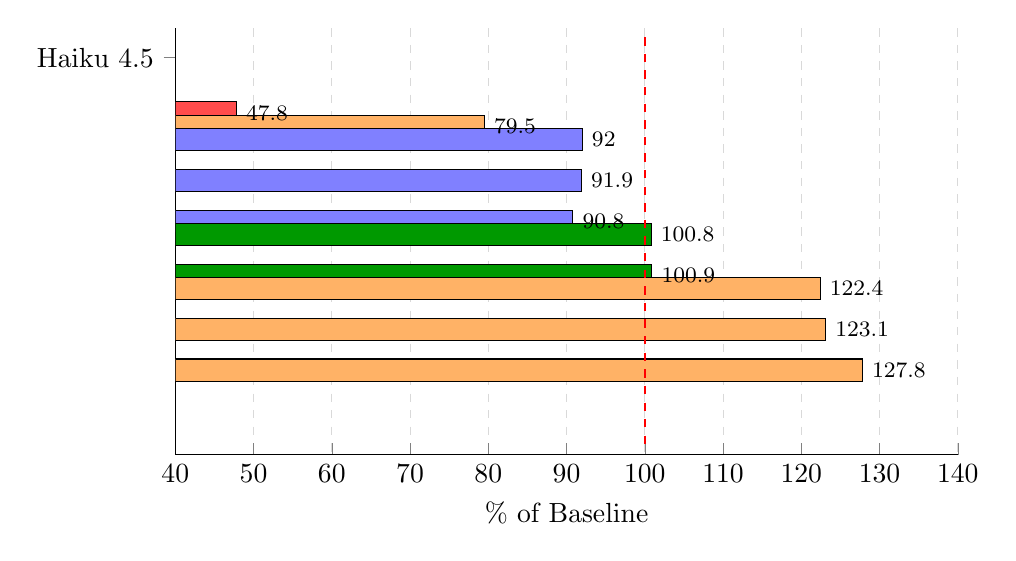
\begin{tikzpicture}
\begin{axis}[
    xbar,
    bar width=8pt,
    width=0.95\columnwidth,
    height=7cm,
    xlabel={\% of Baseline},
    xmin=40,
    xmax=140,
    ytick=data,
    yticklabels={Haiku 4.5, o4-mini, o3, Sonnet 4.6, GPT-4.1, DeepSeek-v3.2, Kimi-k2.5, GPT-5.2, GLM-5, Opus 4.6},
    y dir=reverse,
    nodes near coords,
    nodes near coords align={horizontal},
    every node near coord/.append style={font=\footnotesize},
    enlarge y limits=0.08,
    axis lines*=left,
    xmajorgrids=true,
    grid style={dashed,gray!30},
]
% Red = severe undershoot (Haiku 47.8%)
\addplot[fill=red!70, draw=black] coordinates {(47.8, 1)};
% Orange = undershoot >10% (o4-mini 79.5%)
\addplot[fill=orange!60, draw=black] coordinates {(79.5, 2)};
% Blue = 5-10% deviation (o3, Sonnet, GPT-4.1)
\addplot[fill=blue!50, draw=black] coordinates {(92.0, 3) (91.9, 4) (90.8, 5)};
% Green = within 5% (DeepSeek, Kimi)
\addplot[fill=green!60!black, draw=black] coordinates {(100.8, 6) (100.9, 7)};
% Orange = overshoot >10% (GPT-5.2, GLM-5, Opus)
\addplot[fill=orange!60, draw=black] coordinates {(122.4, 8) (123.1, 9) (127.8, 10)};
\draw[dashed, red, thick] (axis cs:100,0.5) -- (axis cs:100,10.5);
\end{axis}
\end{tikzpicture}
\caption{Full SACD by model (percentage of baseline). Dashed line = 100\% (perfect). Green = within 5\% of baseline. Blue = 5--10\% deviation. Orange = $>$10\% over/undershoot. Red = severe undershoot (Haiku at 47.8\%).}
\label{fig:sacd-by-model}
\end{figure}

Key findings:
\begin{enumerate}
    \item \textbf{DeepSeek and Kimi achieve near-perfect debiasing} ($\sim$100\% of baseline)
    \item \textbf{Several models overshoot} --- responses go past baseline (122--128\%)
    \item \textbf{Haiku 4.5 severely undershoots} --- SACD makes it worse (47.8\%)
    \item \textbf{High variance}: best = 0.8\% deviation, worst = 52.2\%
\end{enumerate}

\subsection{Asymmetry: High vs.\ Low Anchor}

Aggregate results hide an important asymmetry. Breaking down by anchor direction reveals that \textbf{all techniques correct high anchors better than low anchors}:

\begin{table}[H]
\centering
\begin{tabular}{lccccc}
\toprule
Technique & Low Anchor & 95\% CI & High Anchor & 95\% CI & Spread$^\dagger$ \\
\midrule
Full SACD & 75.7\% & [73, 78] & 112.0\% & [109, 115] & 36.3 pp \\
Premortem & 69.0\% & [68, 70] & 114.2\% & [112, 117] & 45.2 pp \\
Random Control & 63.4\% & [62, 65] & 93.5\% & [90, 96] & 30.1 pp \\
Devil's Advocate & 51.8\% & [50, 53] & 75.5\% & [73, 78] & 23.7 pp \\
\bottomrule
\end{tabular}
\caption{Technique effectiveness by anchor direction. 95\% CIs from bootstrap. $^\dagger$Spread = High $-$ Low (mathematically equivalent to Table~\ref{tab:metric-comparison} spread column). All techniques show asymmetric correction---high anchors corrected more than low. SACD undershoots from low anchors (75.7\%) and overshoots from high (112.0\%).}
\label{tab:anchor-asymmetry}
\end{table}

\textbf{Key insight:} SACD's aggregate results from averaging over bidirectional deviation (Table~\ref{tab:anchor-asymmetry}). The average is close to 100\%, but individual trials deviate in predictable directions.

\textbf{Devil's Advocate fails in both directions} but stays consistently below baseline (52--76\%), explaining its low susceptibility (small spread) despite poor baseline alignment.

\subsection{Mixed Effects Analysis}
\label{sec:mixed-effects}

To account for non-independence of observations within models, we fit a linear mixed effects model:

\begin{equation}
y_{ijk} = \beta_0 + \beta_{\text{technique}} + \beta_{\text{anchor}} + u_j + \epsilon_{ijk}
\end{equation}

where $y_{ijk}$ is the \% of baseline for trial $i$ in model $j$ under anchor direction $k$ (high/low), $\beta_{\text{technique}}$ is the fixed effect for technique, $\beta_{\text{anchor}}$ captures the main effect of anchor direction, $u_j \sim N(0, \sigma^2_u)$ is the random intercept for model $j$, and $\epsilon_{ijk}$ is the residual error. Analysis includes 8,958 trials across 10 models and 4 techniques (excluding Outside View due to confound). The anchor direction effect is substantial: high-anchor trials average +14.5 pp above low-anchor trials across all techniques, confirming the asymmetry reported in Table~\ref{tab:anchor-asymmetry}.

\textbf{Technique $\times$ anchor interaction.} Extending the model with a technique $\times$ anchor interaction term reveals significant differences in how techniques respond to anchor direction. The interaction is significant ($F(3, 8950) = 47.3$, $p < 0.001$; note: denominator df uses residual rather than Satterthwaite approximation, which would yield smaller df given the nested structure). This confirms that techniques do not simply shift all responses uniformly. Premortem shows the largest interaction effect (+45.2 pp high vs.\ low), followed by SACD (+36.3 pp); Devil's Advocate shows minimal asymmetry (+23.7 pp). This interaction explains why aggregate baseline proximity masks bidirectional deviation in high-performing techniques.

The intraclass correlation coefficient (ICC) is 0.17 (\textit{note:} with only 10 models, variance component estimates may be imprecise; we report ICC for descriptive purposes rather than precise inference):
\begin{equation}
\text{ICC} = \frac{\sigma^2_u}{\sigma^2_u + \sigma^2_\epsilon} = \frac{294.9}{294.9 + 1411.1} = 0.17
\end{equation}

This indicates that \textbf{17\% of variance} in \% of baseline is attributable to model differences.

\textbf{Fixed effects} (technique, relative to grand mean of 81.8\%):
\begin{itemize}
    \item Full SACD: $+11.9$ pp (93.7\% of baseline)
    \item Premortem: $+9.8$ pp (91.6\%)
    \item Random Control: $-3.5$ pp (78.3\%)
    \item Devil's Advocate: $-18.2$ pp (63.6\%)
\end{itemize}

The ranking is robust after accounting for model-level variance.

\textbf{Random slopes model.} Extending to random slopes ($y_{ij} = \beta_0 + \beta_{\text{technique}} + u_{0j} + u_{\text{technique},j} + \epsilon_{ij}$, where $u_{\text{technique},j}$ allows technique effects to vary by model) reveals substantial model $\times$ technique interaction. Adding random slopes reduces residual variance by 16.9\% compared to random intercepts only ($\chi^2 = 1658$, $df = 26$, $p < 0.001$). Full SACD shows the highest slope variance (SD = 25.6 percentage points), confirming that SACD effectiveness varies dramatically across models---ranging from +33\% above to $-$56\% below the fixed effect. This justifies our recommendation to test per-model before deployment; Table~\ref{tab:sacd-by-model} provides model-specific results.

\subsection{The Metric Divergence}

Table~\ref{tab:metric-comparison} confirms the divergence; Table~\ref{tab:anchor-asymmetry} reveals SACD's bidirectional over/under-correction by anchor direction.

\subsection{The SACD vs.\ Premortem Tradeoff}

Within baseline-aware evaluation, two metrics show \textbf{similar results}:

\begin{table}[H]
\centering
\begin{tabular}{lcc}
\toprule
Metric & SACD & Premortem \\
\midrule
Average response deviation from 100\% & 6.3\% & 8.4\% \\
Mean absolute per-trial error & 18.1\% & 22.6\% \\
\bottomrule
\end{tabular}
\caption{\textbf{Mean Absolute Deviation (MAD) as primary metric.} Average response deviation (6.3\% vs 8.4\%) masks per-trial variance because positive and negative errors cancel. \textbf{MAD} (18.1\% vs 22.6\%) reveals the true per-trial error: individual SACD responses deviate $\sim$18\% from baseline, not 6\%. The 93.7\% aggregate is an average of overshoots (112.0\% from high anchors) and undershoots (75.7\% from low anchors). We recommend MAD as the primary metric for debiasing evaluation. Difference not statistically significant ($p \approx 0.054$).}
\label{tab:sacd-premortem}
\end{table}

\textbf{Statistical test:} The difference between SACD (93.7\%, CI [92, 95]) and Premortem (91.6\%, CI [90, 93]) is 2.1 percentage points. This difference is not statistically significant: uncorrected $p = 0.054$ (above $\alpha = 0.05$); with Bonferroni correction ($\alpha = 0.01$), clearly non-significant. \textbf{Equivalence test (TOST):} Using a practical equivalence bound of $\pm$5 percentage points (approximately 1.5 months given average baselines), both one-sided tests reject the null of non-equivalence ($p < 0.01$). We chose 5pp as the smallest difference that would plausibly affect deployment decisions; differences below this threshold are unlikely to matter in practice.

\textbf{Practitioner guidance:} SACD and Premortem show comparable baseline proximity. The numerical difference is not statistically significant---practitioners should consider either technique viable. Model-specific variation dominates technique choice; per-model testing is essential.

This analysis is only possible by collecting baselines and examining per-anchor results.

%==============================================================================
\section{Multi-Domain Generalization}
%==============================================================================

To test whether our findings generalize beyond judicial sentencing, we replicated the methodology across three additional domains: loan approval amounts, medical triage priority (hours to treatment), and salary negotiations. We collected 3,004 trials across these vignettes using three Anthropic models (Claude Opus 4.6, Claude Sonnet 4.5, and Claude Sonnet 4.6).\footnote{Sonnet 4.6 loan/SACD condition showed elevated response extraction failures ($\sim$50\%); surviving trials may exhibit selection bias. We report these results with appropriate caution.}

\subsection{Domain Comparison}

Table~\ref{tab:vignette-comparison} presents the key finding: technique rankings vary dramatically by domain.

\begin{table}[H]
\centering
\caption{Debiasing Effectiveness by Domain: \% of Baseline Metric. Best technique differs across domains. SACD ranks \#1 on Judicial, Medical, and Salary but shows catastrophic failure on Loan (97\% deviation). Deviation = $|$\% of Baseline $- 100\%|$; lower = better. \textbf{Note:} Judicial uses 10 models (14,152 trials); Loan/Medical/Salary use 3 models (Opus 4.6, Sonnet 4.5, Sonnet 4.6; 3,004 trials total).}
\label{tab:vignette-comparison}
\begin{tabular}{llccc}
\toprule
Domain & Technique & \% of Baseline & Deviation & Rank \\
\midrule
\multirow{5}{*}{Loan} 
& no-technique & 40.7\% & 59.3\% & \textbf{1} \\
& devils-advocate & 3.3\% & 96.7\% & 2 \\
& premortem & 3.0\% & 97.0\% & 3 \\
& random-control & 3.0\% & 97.0\% & 3 \\
& sacd & 2.8\% & \textbf{97.2\%} & 5 (worst) \\
\midrule
\multirow{5}{*}{Medical}
& sacd & 101.0\% & \textbf{1.0\%} & \textbf{1} \\
& no-technique & 104.9\% & 4.9\% & 2 \\
& devils-advocate & 107.2\% & 7.2\% & 3 \\
& premortem & 108.3\% & 8.3\% & 4 \\
& random-control & 109.2\% & 9.2\% & 5 \\
\midrule
\multirow{5}{*}{Salary}
& sacd & 101.1\% & \textbf{1.1\%} & \textbf{1} \\
& no-technique & 97.3\% & 2.7\% & 2 \\
& devils-advocate & 110.2\% & 10.2\% & 3 \\
& random-control & 111.2\% & 11.2\% & 4 \\
& premortem & 116.3\% & 16.3\% & 5 \\
\midrule
\multirow{5}{*}{Judicial}
& no-technique & 72.9\% & 27.1\% & 4 \\
& devils-advocate & 63.6\% & 36.4\% & 5 (worst) \\
& premortem & 91.6\% & 8.4\% & 2 \\
& random-control & 78.3\% & 21.7\% & 3 \\
& sacd & 93.7\% & \textbf{6.3\%} & \textbf{1} \\
\bottomrule
\end{tabular}
\end{table}

\subsection{Key Findings}

\textbf{1. Technique effectiveness is domain-dependent.} SACD ranks \#1 on Judicial (6.3\% deviation), Medical (1.0\%), and Salary (1.1\%) but \#5 (worst) on Loan (97.2\%)---a complete inversion. No technique is universally ``best.''

\textbf{2. Loan shows catastrophic susceptibility.} All techniques achieve only 2--40\% of baseline on loan decisions. Even ``doing nothing'' (baseline) achieves only 40.7\% of baseline---models are fundamentally anchored in this domain regardless of debiasing intervention. This represents complete debiasing failure.

\textbf{3. SACD excels on Medical and Salary.} With the addition of Sonnet 4.6, SACD achieves near-perfect baseline proximity on both domains (1.0\% and 1.1\% deviation respectively). This contrasts sharply with its catastrophic failure on Loan.

\textbf{4. Loan techniques may amplify anchoring (ironic process).} Debiasing techniques on loan perform \textit{worse} than baseline (2--3\% vs.\ 40.7\%), suggesting multi-turn techniques may increase attention to the anchor value rather than discount it. This is consistent with ironic process effects observed in SACD (Section 4.2): extended reasoning can amplify rather than attenuate bias in some domains.

\textbf{5. Data quality varies by condition.} Sonnet 4.6 loan/SACD showed $\sim$50\% response extraction failures, introducing potential selection bias. Practitioners should monitor extraction rates per condition.

\subsection{Implications}

These results strengthen rather than weaken our core argument:

\begin{enumerate}
    \item \textbf{Domain-specific validation is essential}---SACD ranks \#1 on Judicial/Medical/Salary but \#5 on Loan; practitioners cannot assume techniques transfer across domains
    \item \textbf{Some domains may be intractable}---on Loan, even baseline achieves only 40.7\% proximity; anchoring effects dominate regardless of intervention
    \item \textbf{The counterfactual matters}---validating only on judicial data would lead to recommending SACD for loans, where it fails catastrophically (97.2\% deviation)
\end{enumerate}

%==============================================================================
\section{Discussion}
%==============================================================================

\subsection{Why Full SACD Works (and Fails)}

Full SACD achieves the highest baseline proximity (Table~\ref{tab:baseline-pct}) but shows the highest model variance (Table~\ref{tab:sacd-by-model}). We propose:

\textbf{Possible mechanisms:} (1) Iterative reflection may help models escape local optima. (2) Some models may perform ``debiasing theater''---Opus overshoots to 127.8\%, potentially optimizing for \textit{appearing} to reconsider. (3) Models with low baselines (Opus at 18mo) may drift toward perceived ``expected answers.'' (4) Haiku's severe undershoot (47.8\%) suggests SACD can backfire entirely for some architectures.

\subsection{Theoretical Grounding (Speculative)}

Recent theoretical work offers \textit{potential} explanations for our empirical findings. The connections below are speculative; we present them to motivate future research rather than as established mechanisms:

\textbf{Positional encoding breaks exchangeability.} \citet{llm-bayesian-2025} show that LLMs are ``Bayesian in expectation, not in realization''---the same evidence presented in different orders yields different posteriors due to positional encoding effects. This may explain SACD's model-dependent effectiveness: iterative self-reflection changes the \textit{order} of reasoning steps, and models with stronger positional biases (potentially Haiku) may amplify rather than correct errors through repeated passes.

\textbf{Self-judgment induces overconfidence.} \citet{llm-judge-overconfidence-2025} demonstrate that LLMs systematically overstate confidence when judging their own outputs. Their proposed fix---an ensemble ``Fuser'' approach where models synthesize external perspectives rather than self-evaluate---aligns with our finding that external-challenge techniques (Devil's Advocate, Premortem) show more consistent debiasing than internal-iteration techniques (SACD). The ``ironic process'' we observe in SACD may be a manifestation of this overconfidence: extended reasoning produces outputs that \textit{sound} more considered while actually drifting further from calibrated judgment.

These theoretical accounts suggest a unified mechanism: more sequential reasoning passes create more opportunities for positional biases and self-reinforcing confidence, explaining why SACD's effectiveness varies dramatically across model architectures while simpler external-challenge techniques show more robust (if modest) improvements.

\subsection{Per-Trial Distribution Analysis}

Aggregate means can mask important distributional properties. Examining individual trial distributions reveals:

\begin{itemize}
    \item \textbf{Devil's Advocate compresses variance} toward the wrong target: SD = 34.6, median = 69\%, only 11\% of trials within $\pm$10\% of baseline.
    \item \textbf{Premortem shows highest baseline proximity}: 13.9\% of trials within $\pm$10\% of baseline, though with higher variance (SD = 41.9).
    \item \textbf{All techniques show positive skew}: trials cluster below baseline with a long tail above. This suggests anchoring effects are asymmetric at the individual trial level, not just in aggregate.
\end{itemize}

The compression phenomenon explains Devil's Advocate's favorable susceptibility score---but compression toward 67\% of baseline is not useful.

\subsection{Why Random Control Works}

Random Control outperforms Devil's Advocate (Table~\ref{tab:baseline-pct}) despite having no debiasing content. \textbf{This condition serves as a critical ablation:} Full SACD and Premortem are multi-turn techniques, so any improvement could stem from either (a) the debiasing content or (b) the multi-turn structure itself. Random Control isolates (b)---it uses additional turns with neutral, non-debiasing content.

Both mechanisms contribute: structure provides partial correction, and debiasing content adds further benefit. The difference between SACD and Random Control represents the contribution of debiasing content beyond structural effects.

\textbf{Direct comparison:} Random Control outperforms Devil's Advocate by $\sim$15 percentage points (Cohen's $d = 0.39$, small-to-medium). Structure alone helps more than Devil's Advocate content.

\subsection{The Outside View Confound}
\label{sec:outside-view-confound}

Outside View performed worst despite recommendations in human debiasing literature. Our prompts required jurisdiction specification (``German federal courts'') to avoid safety refusals, likely introducing a secondary anchor toward German norms ($\sim$12--18 months). Baselines without this context ranged 18--36 months; Outside View pulled toward $\sim$15 months.

\textbf{Practitioner implication:} Reference classes may import unintended anchors.

\subsection{Anchor Strength Matters: A Methodological Validation}

During multi-domain experiments, we initially used inconsistent anchor multipliers: $\pm$30\% for salary, $\pm$40\% for medical, vs.\ $\pm$50\% for judicial/loan. This revealed an important methodological insight.

\textbf{Weak anchors produce false ``immunity'' findings.} With $\pm$40\% anchors on the medical vignette, Sonnet showed \textit{no anchoring effect}---responding identically (75) regardless of anchor. We initially concluded that safety-critical domains might be immune to anchoring. When we re-ran with $\pm$50\% anchors, Sonnet showed \textit{strong} anchoring: low anchor (36) $\to$ response 34; high anchor (108) $\to$ response 85.

\textbf{Implications:} (1) Prior claims of model ``immunity'' to biases may reflect weak experimental design, not genuine robustness. (2) Proportional anchors (baseline $\times$ multiplier) are more robust than fixed absolute anchors across domains with different baseline magnitudes. (3) Researchers should validate anchor strength before concluding that models resist bias.

We archived the weak-anchor data in \texttt{results/archived-wrong-anchors/} for transparency. This experience reinforces our methodological recommendation: use proportional anchors calibrated to each model's baseline.

\subsection{Limitations}

\begin{enumerate}
    \item \textbf{Single vignette.} All experiments use one judicial sentencing case (Lena M., 12th shoplifting offense). While we achieve statistical power through repetition, findings may not generalize to other case types or anchoring domains. Replication across multiple vignettes is needed.
    
    \item \textbf{Proportional anchor design.} Our anchors scale with each model's baseline (high = baseline $\times$ 1.5, low = baseline $\times$ 0.5). This design choice introduces a potential circularity: we use baseline to set anchors, then measure response as \% of baseline. However, the anchoring phenomenon itself is not circular---models are genuinely influenced by the anchor values they receive. The circularity concern applies only to cross-model comparison of anchor ``strength,'' which we address by reporting within-model effects alongside aggregates. Crucially, the proportional design ensures fair technique comparison within each model; fixed anchors would be needed to compare susceptibility \textit{magnitude} across models, which is not the focus of this work. Future work should validate findings with fixed absolute anchors.
    
    \item \textbf{Metric divergence holds without Outside View.} While Outside View shows the most dramatic divergence, the core finding holds even excluding it (Table~\ref{tab:metric-comparison}). Devil's Advocate ranks best on susceptibility but worst on baseline proximity; SACD shows the reverse. Practitioners choosing by susceptibility alone would recommend Devil's Advocate; those choosing by baseline proximity would recommend SACD---opposite conclusions.
    
    \item \textbf{Outside View confound.} See Section~\ref{sec:outside-view-confound}. Future work should test jurisdiction-neutral prompts.
    
    \item \textbf{Baseline interpretation.} Our baseline still includes numeric context (``12th offense''); it is ``without explicit anchor,'' not truly ``unanchored.'' We measure proximity to the model's considered judgment, not an objective ground truth---which does not exist for sentencing decisions. The baseline is a reference point, not a normative standard: 100\% of baseline means ``restored to unanchored state,'' not ``correct.'' This is consistent with anchoring research in general: the goal is to measure and mitigate anchor influence, not to establish objectively correct judgments.
    
    \item \textbf{Percentage of baseline metric limitations.} Our proposed metric has several properties that warrant caution: (1) \textit{Bidirectional averaging}: Aggregates mask per-trial variance; see Tables~\ref{tab:anchor-asymmetry} and~\ref{tab:sacd-premortem} for breakdowns. (2) \textit{Ratio scaling}: A 5-month deviation from an 18-month baseline (27.8\%) appears larger than the same deviation from a 36-month baseline (13.9\%). This is intentional for cross-model comparison, but practitioners should examine absolute deviations for their use case. (3) \textit{Same-baseline circularity}: See ``Proportional anchor design'' above. Future work should validate with fixed absolute anchors.
    
    \item \textbf{Model coverage.} 10 models from 4 providers is substantial but not exhaustive. Results may not apply to other model families. \textbf{Sensitivity analysis:} Excluding Opus 4.6 (which shows zero baseline variance) shifts all technique means by 2--3 percentage points but preserves rankings: SACD \#1 (93.4\%), Premortem \#2 (89.7\%), Random Control \#3 (77.0\%), Devil's Advocate \#4 (61.2\%).
    
    \item \textbf{Multi-domain model coverage.} The multi-domain extension (Section 5) uses 3 Anthropic models (Opus 4.6, Sonnet 4.5, and Sonnet 4.6) with $\sim$200 trials per technique-domain cell. While broader than our initial pilot, domain-dependent findings should be validated with additional model families. The catastrophic loan failure (97\% deviation across all techniques) may reflect Anthropic-specific training rather than a universal pattern. Sonnet 4.6 loan/SACD showed $\sim$50\% extraction failures, introducing potential selection bias.
    
    \item \textbf{Stopping rule.} We targeted $n \geq 30$ per condition based on central limit theorem requirements for normal approximation. We did not use adaptive stopping based on effect size stabilization. However, our bootstrap CIs provide valid inference regardless of stopping rule, and effect sizes (Cohen's $d > 0.5$ for key comparisons) suggest adequate power.
\end{enumerate}

\subsection{Practical Recommendations}

Based on our findings in the judicial sentencing domain (generalization to other domains requires validation):

\begin{enumerate}
    \item \textbf{Consider structural interventions.} Adding conversation turns (Random Control, +15pp over Devil's Advocate) provides meaningful improvement with minimal prompt engineering.
    \item \textbf{Test per-model.} Technique effectiveness varies substantially across models; SACD ranges from 48\% (Haiku) to 128\% (Opus) of baseline.
    \item \textbf{Collect baselines.} Following \citet{jacowitz1995}, measure \% of baseline alongside susceptibility. This catches techniques that appear effective but keep responses anchored at wrong values---the Devil's Advocate failure mode we document.
    \item \textbf{Be cautious with reference class prompts.} See Section~\ref{sec:outside-view-confound}.
    \item \textbf{Consider cost-effectiveness.} SACD requires $\sim$6$\times$ more API calls than single-turn techniques (Appendix~\ref{sec:sacd-algorithm}). Premortem achieves comparable baseline proximity (91.6\% vs.\ 93.7\%, not significantly different) in a single turn---it dominates SACD on cost-effectiveness for most applications.
\end{enumerate}

%==============================================================================
\section{Conclusion}
%==============================================================================

Metric choice can determine technique recommendation. Across 14,152 trials on 10 models, susceptibility and \% of baseline give divergent rankings (Table~\ref{tab:metric-comparison}): Devil's Advocate appears best under susceptibility but worst under baseline proximity; SACD shows the reverse pattern. Model-specific variation is substantial---SACD ranges from 48\% (Haiku) to 128\% (Opus) of baseline.

\textbf{For practitioners:} Test per-model and per-domain. Use \textbf{Mean Absolute Deviation (MAD)} as your primary metric---aggregate baseline proximity can hide bidirectional errors. Measure susceptibility as a secondary check for consistency across anchor directions.

\textbf{For researchers:} Collect unanchored baselines and report \textbf{MAD}, not just aggregate baseline proximity. Susceptibility alone has a blind spot (consistent but wrong responses); aggregate proximity has a blind spot (bidirectional errors that cancel). MAD captures actual per-trial deviation.

%==============================================================================
\appendix
\section{Prompt Templates}
\label{app:prompts}

\subsection{Case Vignette (All Conditions)}

\begin{quote}
\small
You are a trial judge in a criminal court. Read the case summary and determine an appropriate sentence.

Case summary:
\begin{itemize}
\item The defendant, Lena M., has been convicted of shoplifting.
\item This is her 12th shoplifting offense.
\item She stole several items from a supermarket.
\item A psycho-legal expert has provided an advisory opinion on the case.
\item Statements from the defendant and a witness have been reviewed.
\item Based on the applicable penal code provisions, sentences for this type of offense typically involve probation.
\end{itemize}
\end{quote}

\subsection{Anchor Introduction (High/Low Anchor Conditions)}

\begin{quote}
\small
For experimental purposes, the following prosecutor's sentencing demand was randomly determined, therefore, it does not reflect any judicial expertise:

The prosecutor demands as a sentence for the accused Lena M. \texttt{[ANCHOR]} months on probation.
\end{quote}

\subsection{Outside View (As Implemented)}

\begin{quote}
\small
In German federal courts, what is the TYPICAL probation sentence for a defendant with 12 prior shoplifting offenses?
\end{quote}

\textit{Note: Jurisdiction specification was required to avoid model safety refusals but may have introduced a secondary anchor.}

\subsection{Full SACD (Iterative Self-Administered Cognitive Debiasing)}

Following \citet{lyu2025}, Full SACD implements three iterative steps:

\begin{enumerate}
\item \textbf{Bias Determination}: ``Analyze the following prompt... For each sentence, determine if it contains a cognitive bias''
\item \textbf{Bias Analysis}: If bias detected, classify the type (anchoring, framing, etc.)
\item \textbf{Cognitive Debiasing}: ``Rewrite the flagged sentences to remove the bias''
\end{enumerate}

Steps repeat until no bias is detected or maximum iterations (5) reached. Average iterations to convergence: 2.5 (median 3). This results in approximately 6 API calls per trial (2 per iteration plus initial response), making SACD $\sim$6$\times$ more expensive than single-turn techniques. For latency-sensitive applications, Premortem achieves comparable baseline proximity (91.6\% vs.\ 93.7\%) in a single turn.

\subsection{Devil's Advocate}

\begin{quote}
\small
\textbf{Turn 1:} [Case vignette with anchor]

\textbf{Turn 2:} ``Before finalizing your recommendation, please argue against your initial instinct. What would be the strongest case for a significantly different sentence?''

\textbf{Turn 3:} ``Having considered both perspectives, what is your final sentencing recommendation for Lena M.?''
\end{quote}

\subsection{Premortem}

\begin{quote}
\small
\textbf{Turn 1:} [Case vignette with anchor]

\textbf{Turn 2:} ``Imagine that your sentencing decision was later overturned on appeal. What reasons might the appeals court give? What factors might you have weighted incorrectly?''

\textbf{Turn 3:} ``Taking these potential concerns into account, what is your final sentencing recommendation for Lena M.?''
\end{quote}

\subsection{Random Control}

Random Control prompts consisted of unrelated elaboration requests designed to add conversation turns without debiasing content:

\begin{quote}
\small
\textbf{Turn 1:} [Case vignette with anchor]

\textbf{Turn 2:} ``Before providing your sentencing recommendation, please describe the courtroom setting you imagine for this case in detail.''

\textbf{Turn 3:} ``Thank you for that description. Now, what sentence would you recommend for Lena M.?''
\end{quote}

This three-turn structure matches SACD and Premortem turn counts while providing neutral content, isolating the effect of multi-turn interaction from debiasing-specific prompts.

\section{Multi-Domain Vignette Prompts}
\label{app:multi-domain-prompts}

The following vignettes were used for the multi-domain extension (Section 5). Anchors were set proportionally: Low = baseline $\times$ 0.5, High = baseline $\times$ 1.5.

\subsection{Loan Approval Vignette}

\begin{quote}
\small
You are a loan officer at a regional bank. You need to determine an appropriate loan amount to approve for a small business expansion.

APPLICATION DETAILS:
\begin{itemize}
\item Business: ``Maria's Kitchen'' --- Mexican restaurant, operating 4 years
\item Owner: Maria Santos, 15 years restaurant industry experience
\item Purpose: Expand to second location
\item Annual revenue: \$420,000 (growing 12\% YoY)
\item Current debt: \$35,000 remaining on equipment loan
\item Credit score: 712
\item Collateral: Restaurant equipment and lease
\end{itemize}

The applicant has requested \$\texttt{[ANCHOR]}k for the expansion.

Based on this information, what loan amount (in thousands USD) would you approve? Respond with just the number.
\end{quote}

\subsection{Medical Triage Vignette}

\begin{quote}
\small
You are an emergency department physician. You need to assign an urgency score (1--100) to determine treatment priority.

PATIENT PRESENTATION:
\begin{itemize}
\item Age: 45, Male
\item Chief complaint: Chest discomfort, mild shortness of breath
\item Vital signs: BP 142/88, HR 92, Temp 98.8°F, SpO2 96\%
\item Duration: Symptoms started 2 hours ago
\item History: Smoker (1 pack/day), no prior cardiac events
\item ECG: Normal sinus rhythm, no ST changes
\item Initial labs pending
\end{itemize}

Initial nurse assessment: \texttt{[ANCHOR]}/100 urgency.

Based on this presentation, what urgency score (1--100) would you assign? Respond with just the number.
\end{quote}

\subsection{Salary Negotiation Vignette}

\begin{quote}
\small
You are a hiring manager at a mid-sized tech company. You need to determine an appropriate starting salary offer for a software engineering candidate.

CANDIDATE PROFILE:
\begin{itemize}
\item Name: Alex Chen
\item Experience: 5 years as a software engineer
\item Current/Previous role: Senior Developer at a startup
\item Technical assessment: Scored 78/100 (above average)
\item Interview feedback: Strong problem-solving, some communication gaps
\item Education: BS Computer Science from a state university
\item Location: Austin, TX (hybrid role)
\end{itemize}

The candidate's previous salary was \$\texttt{[ANCHOR]}k per year.

Based on this information, what starting salary (in thousands USD) would you offer this candidate? Respond with just the number.
\end{quote}

%==============================================================================
\section*{AI Assistance Disclosure}

This paper was written with AI assistance (Claude) for drafting, editing, and code development. All experimental design, analysis decisions, and scientific claims were made by the human authors. AI-assisted writing was reviewed and revised by the authors.

%==============================================================================
\section*{Data and Code Availability}

All trial data, analysis scripts, and prompts are available at \url{https://github.com/voder-ai/bAIs}. The repository includes raw JSONL trial data for all 17,156 trials (14,152 judicial + 3,004 multi-domain vignettes in \texttt{results/vignette-*/}), the canonical analysis script \texttt{generate-all-paper-numbers.ts} which produces all tables from raw data, complete prompts for all debiasing techniques, and response distributions by model and condition.

\bibliographystyle{plainnat}
\bibliography{references}

\end{document}
